%!TEX root = main.tex

% \documentclass[11pt, oneside]{article}   	% use "amsart" instead of "article" for AMSLaTeX format
% \usepackage{geometry}                		% See geometry.pdf to learn the layout options. There are lots.
% \geometry{letterpaper}                   		% ... or a4paper or a5paper or ... 
% \usepackage{graphicx}				% Use pdf, png, jpg, or eps with pdflatex; use eps in DVI mode
% 								% TeX will automatically convert eps --> pdf in pdflatex		
% \usepackage{amssymb}
% \usepackage{natbib}
% \usepackage{amsmath}

% \usepackage{algorithm} % for algorithm
% \usepackage{amsfonts} % for \mathbb{R}

% \begin{document}


\section{Introduction}


The recognition of handwritten digit strings is relevant in a variety of applications in our daily life.
In post office, handwritten ZIP code can be recognized automatically.
At primary school, the grading of arithmetic problems can be completed in one second with a smart phone application.
However, there are still several challenges in this field.
One bottleneck is related with the segmentation module, which segments a string of characters into individual one.
The reason behind is that strings sometimes are not neatly written, e.g. overlapping, touching, and intersecting (\autoref{example}).
Many algorithms have been proposed to deal with this problem.
They can mainly be divided into two categories \citep{casey1996}.
The first one is segmentation-recognition, which means segmentation is completed before recognition.
The second one is recognition based, where the algorithm yields a list of segmentation hypotheses and then assesses each of them through the recognition process.
This method will take the information of the foreground and background into account.
Recently, segmentation-free methods are also introduced \citep{hochuli2018}.

\begin{figure}[ht] %  figure placement: here, top, bottom, or page
   \centering
   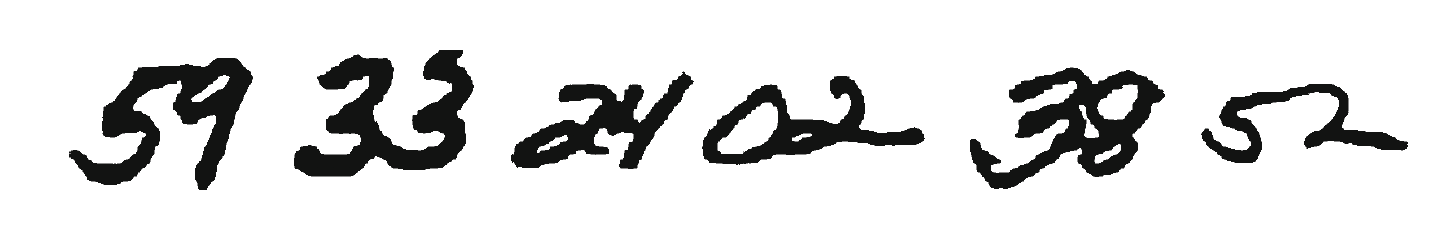
\includegraphics[width=2in]{example.png} 
   \caption{Variability of connections between handwritten digits.}
   \label{example}
\end{figure}

In this project, the main goal is to deal with the intersections in the handwritten digit strings.
Here we will focus on segmentation-recognition implementing the spectral clustering based on local principle component analysis (PCA) \citep{arias2017}.
A straightforward idea for segmentation is to utilize spectral clustering \citep{ng2002}.
However, a fatal drawback of spectral clustering is that it cannot separate two intersecting clusters.
Thus, it cannot deal with the segmentation in handwritten digits.
\citet{shashua2006} claim that a multiway affinity is needed to capture complex structure in data (e.g. intersection) beyond proximity attributes.
\citet{fan2006} first implemented subspace clustering based on local PCA.
Later, \citet{goldberg2009} developed a spectral clustering method within a semi-supervised learning framework.
Continuing this line of work, \citep{arias2011} suggest a spectral clustering method based on the estimation of the local linear structure (tangent bundle) via local PCA.
There are also two concurrent publications \citep{wang2011, gong2012} with quite similar methods.

The rest of the paper is organized as follows.
In Section 2, we will show authors' algorithms to implement spectral clustering based on local PCA.
The rationale behind the algorithm will be briefly discussed.
In Section 3, we will analyze the results of the algorithm.
In Section 4, we will show one application of this algorithm.
We will build a auto-grader for arithmetic problems.
This is also the motivation of this project.
With a photo of a set of arithmetic problems, our program can grade all problems.  

\section{Methodology}
% \makeatletter
% \renewcommand{\thealgorithm}{} % remove Algorithm number such as Algorithm "4"
% \makeatother
% \begin{algorithm}[htbp]
% \caption{Spectral Clustering Based on Local PCA}
\vspace{0.1in}
\textbf{Input:} \newline
Data points $\boldsymbol{x}_1, ..., \boldsymbol{x}_n \in \mathbb{R}^D$; neighborhood radius $r>0$; spatial scale $\epsilon>0$; projection scale $\eta>0$; intrinsic dimension $d$; number of clusters $K$. \vspace{0.1in} \newline
\textbf{Steps:  (called ``Algorithm 4" in the paper)}
\begin{enumerate}
\item Pick one point $\boldsymbol{y}_1$ at random from the data.
Pick another point $\boldsymbol{y}_2$ among the data points not included in neighborhood $N_r(\boldsymbol{y}_1)$, and repeat the process, selecting centers $\boldsymbol{y}_1$, ..., $\boldsymbol{y}_{n_0}$.
Here we define the neighborhood $N_r(\boldsymbol{x})=\{\boldsymbol{x}_j : ||\boldsymbol{x}-\boldsymbol{x}_j|| \leqslant r\}$ for any point $\boldsymbol{x} \in \mathbb{R}^D$ and $r>0$, given a data set $\boldsymbol{x}_1, ..., \boldsymbol{x}_n$.
\item For each $i$ = 1, ..., $n_0$, compute the sample covariance matrix $\boldsymbol{C}_i$ of $N_r(\boldsymbol{y}_i)$.
Let $\boldsymbol{Q}_i$ denote the orthogonal projection onto the space spanned by the top $d$ eigenvectors of $\boldsymbol{C}_i$.
\item Compute the following affinities between center pairs:
\begin{equation}
W_{ij}=\exp \left( -\frac{||\boldsymbol{y}_i-\boldsymbol{y}_j||^2}{\epsilon^2} \right) \cdot \exp \left(-\frac{||\boldsymbol{Q}_i-\boldsymbol{Q}_j||^2}{\eta^2} \right)
\end{equation}
\item (Spectral Graph Partitioning) Compute $\boldsymbol{Z} = (Z_{ij})$ according to $Z_{ij} = W_{ij}/\sqrt{\Delta_i \Delta_j}$, with $\Delta_i=\Sigma_{j=1}^{n} W_{ij}$.
Extract the top $K$ eigenvectors of $Z$.
Renormalize each row of the resulting $n \times K$ matrix.
Apply $K$-means to the row vectors.
\item The data points are clustered according to the closest center in Euclidean distance.
\end{enumerate}
% \end{algorithm}
\vspace{1em}
The main idea is that we first divide the original data points into small circles (or spheres) $N(\boldsymbol{y}_i)$ with the radius $r$.
Then we grab the information about the direction of the local data arrangement in each circle through the sample covariance matrix $\boldsymbol{C}_i$ and extract the information as the projection matrix $\boldsymbol{Q}_i$.
The affinities $W_{ij}$ are set so that circles are classified as the same cluster if they are geometrically close and the local directions of the data arrangement are similar.

\autoref{cross} is the simplest example of the clustering by this algorithm ($K = 2$, $r = 15.0$, $\epsilon = 15.0$, $\eta = 0.5$).
The cross-shaped data is seccessfully separated by the intersection.

\begin{figure}[htbp]
\centering
\vspace{-1em}
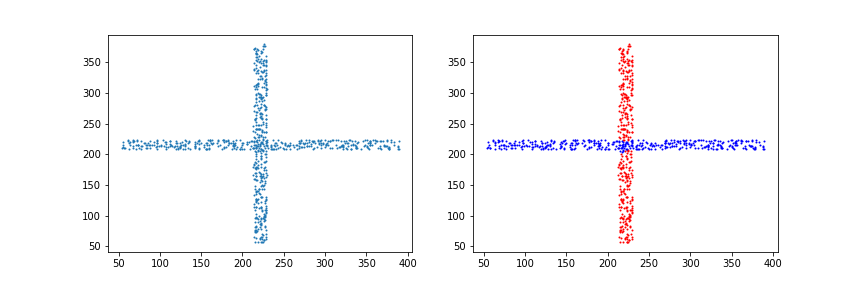
\includegraphics[width=0.8  \textwidth]{cross_shaped.png}
\vspace{-1em}
\caption{Clustering example}
\label{cross}
\end{figure}


% \end{document}  